\documentclass{llncs}
%\pagestyle{headings} %page numbers
%\usepackage[font=small,labelfont=bf]{caption}


%% Language and font encodings
\usepackage[english]{babel}
\usepackage[utf8x]{inputenc}
\usepackage[T1]{fontenc}
\usepackage[outdir=./]{epstopdf}

\usepackage[]{xcolor}
%% Sets page size and margins
\usepackage[a4paper,top=3cm,bottom=2cm,left=3cm,right=3cm,marginparwidth=1.75cm]{geometry}

%% Useful packages
%\usepackage{amsmath}
\usepackage{graphicx}

\usepackage[colorinlistoftodos]{todonotes}
\title{Super awesome embeddings}
\author{Grzegorz Beringer \and Mateusz Jabłoński \and Piotr Januszewski \and Julian Szymański}
%

 \institute{
Faculty of Electronic Telecommunications and Informatics\\
Gda{\'n}sk University of Technology, Gda{\'n}sk, Poland
}

% (feature abused for this document to repeat the title also on left hand pages)

% the affiliations are given next; don't give your e-mail address
% unless you accept that it will be published
%\institute{Faculty of Electronics,
%Telecommunications and Informatics,
%Gdańsk University of Technology,
%ul. Narutowicza 11/12, 80-952 Gdańsk,
%Poland}

\begin{document}
\maketitle
\begin{abstract}

In recent years word embeddings have been shown to boost the performance in NLP tasks such as syntactic parsing or sentiment analysis, but also in multimodal systems like image captioning or visual question answering.
It is therefore not surprising that word embeddings have been applied to Word Sense Disambiguation (WSD) problem as well.
In this work, we present how a simple word embeddings average-based method can be used to produce keyword (meaning) and context embeddings, and how the former can be improved with two embeddings distance optimization techniques.
We also open source the dataset that was created for the purpose of this research.
It is composed of 6 ambiguous words, with 4 to 7 meanings each, and collected real-world usage examples of those meanings, with tagged words to be disambiguated.

\keywords{word sense disambiguation, word embeddings}
\end{abstract}

\section{Introduction}
\label{introduction}

Word Sense Disambiguation (WSD) is an open problem of natural language processing (NLP) and ontology. WSD is identifying which sense of a word (i.e. meaning) is used in a sentence based on the word context. Difficulty is when the word has multiple meanings (e.g. a decision tree, a tree data structure, a tree in a forest). The problem requires two inputs: a dictionary to specify the senses which are to be disambiguated and a corpus of language data to be disambiguated. WSD task has two variants: "lexical sample" and "all words" task. The former aim to disambiguate the occurrences of a small sample of selected target words, while in the latter all the words in a piece of running text need to be disambiguated. Our solution targets the former one, but could be extended to the latter variant.
The solution to WSD would be useful in many NLP related problems as: relevance of search engines, anaphora resolution, coherence, inference, etc.

Word embeddings are a product of feature learning techniques in NLP, where words from the vocabulary are mapped to vectors of real numbers. Conceptually it involves a dimensionality reduction from a space with one dimension per word to a continuous vector space with a much lower dimension.
Methods to generate this mapping include artificial neural networks\cite{word2vec}\cite{GloVe}\cite{fastText}, dimensionality reduction on the word co-occurrence matrix\cite{Levy2014NWE} and probabilistic models\cite{Globerson2007EEC}.
Word embeddings are commonly used as the input representation. They have been shown to boost the performance in NLP tasks such as syntactic parsing\cite{parsingGrammars} and sentiment analysis\cite{sentimentAnalysis}.

Word embeddings cannot distinguish between different meanings of ambiguous words by themselves. By definition, there is only one embedding for each word e.g. for word ``tree'' there is a single real-valued vector. What can be done, is to try to distinguish the meaning based on the context, in which the word was used. Then, we treat each meaning as a separate keyword, which has its own embedding.
We propose a simple method to infer the word meaning: an average of the context and the word embeddings and number of improvements to this approach in the chapter ``Our method''. Experiments with our solution are presented in the chapter ``Experiments''. To conduct those experiments we have created the dataset composed of 6 ambiguous words, with 4 to 7 meanings each, and collected real-world usage examples of those meanings, with tagged words to be disambiguated. We describe our dataset in the chapter ``Dataset''. In the chapter ``Related work'' we present other approaches to WSD.

\section{Related work}
\label{related work}

\section{Dataset}
\label{dataset}
For the purpose of testing word embeddings as a method to differentiate between different meanings, we gathered examples for 6 ambiguous words, 4-7 meanings each (28 meanings in total).
Ambiguous word together with its meaning constitues a \textit{keyword}, which we use as a separate class when identyfing the closest meaning given some context.
All keywords can be seen on Figure 1.

\begin{figure}
    \label{fig:keywords}
    \caption{Ambiguous words with their meanings (keywords) from the dataset}
    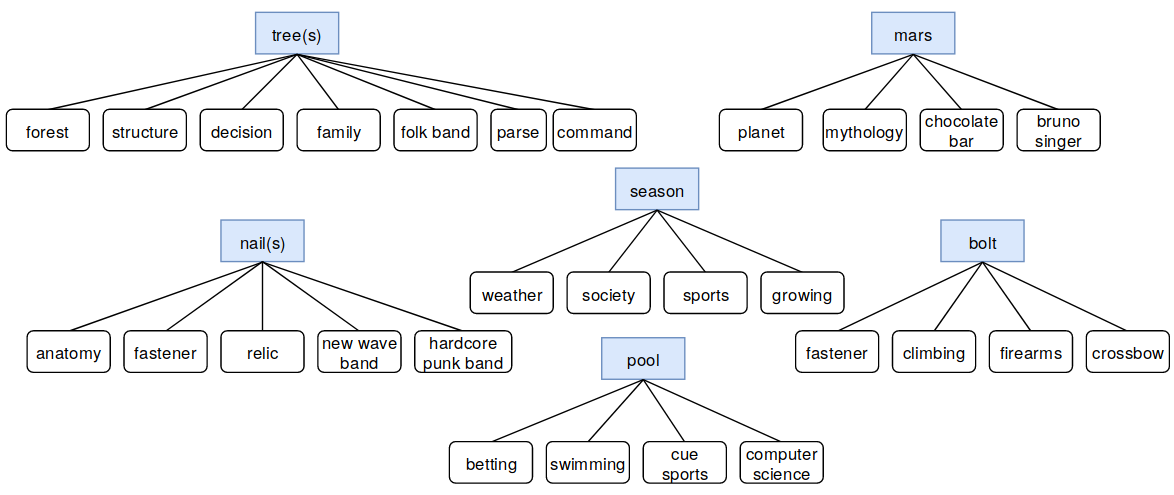
\includegraphics[scale=0.35]{res/keywords.png}
\end{figure}

Examples were mostly gathered from Wikipedia, using \textit{What links here} utility for each keyword.
If usage examples from Wikipedia were not enough, other websites were used (or even the Wikipedia article on specific keyword itself).

The dataset is split into training and test set, with 5 training and 10 test examples for each keyword.
Each example is stored in plain text, with the ambiguous word marked with "*" on both sides.

The correct keyword for each example, together with a path to file and a link, where the original text was taken from, are stored in CSV files: \textit{train.csv} for training set, \textit{test.csv} for test set (columns: path,keyword,link).
Keywords themselves, together with links to their Wikipedia articles, are stored in \textit{keywords.csv} file.
Dataset, together with the code to execute experiments from this paper, can be found on our GitHub repository \cite{repository}.

\bigskip
\underline{Example for \textit{bolt crossbow} keyword:}

\smallskip
\textbf{Keyword definition}: keyword.csv\newline
\textit{
keyword,link\newline
...\newline
bolt crossbow,https://en.wikipedia.org/wiki/Crossbow\_bolt\newline}

\smallskip
\textbf{Test set}: test.csv\newline
\textit{
path,keyword,link\newline
...\newline
texts/test/bolt\_crossbow\_5.txt,bolt crossbow,https://en.wikipedia.org/wiki/Incendiary\_device\newline
}

\smallskip
\textbf{Text}: texts/test/bolt\_crossbow\_5.txt\newline
\textit{"Sulfur- and oil-soaked materials were sometimes ignited and thrown at the enemy, or attached to spears, arrow and *bolts* and fired by hand or machine. Some siege techniques—such as mining and boring—relied on combustibles and fire to complete the collapse of walls and structures."}

\bibliographystyle{splncs}
\bibliography{sample}

\end{document}


\begin{thebibliography}

\end{thebibliography}
